\subsection{Caso resuelto}
El caso que se va realizar es la personalización de un contenedor y una imagen basada en ubuntu instalando el servidor Apache Web Server.

Para realizar la descarga de la imagen correspondiente se utiliza el comando

\begin{commandshell} docker pull ubuntu \end{commandshell}

Paso siguiente se crea un nuevo contenedor con el nombre de ubuntu-apache iniciando una consola interactiva, de la siguiente forma

\begin{commandshell} docker run --name ubuntu-apache -it ubuntu /bin/bash \end{commandshell}

Al estar en la terminal del contenedor se ejecutan los siguientes comandos para la instalación del servicio web de la siguiente forma 
\begin{commandshellroot}
apt update
apt install apache2
service start apache2
\end{commandshellroot}

Luego de instalados los paquetes necesarios e iniciado el servicio, se debe volver a la terminal del host y crear una imagen a partir del contenedor modificado previamente utilizando el siguiente comando

\begin{commandshell}
docker commit -c='CMD ["apache2ctl" , "-DFOREGROUND"]' \\
    -c 'EXPOSE 80' ubuntu-apache imagen-apache
\end{commandshell}

En el comando mostrado anteriormente, se realizan dos modificaciones importantes a la imagen: 
\begin{itemize}
    \item -c='CMD ["apache2ctl" , "-DFOREGROUND"]': Se agrega que al momento de su inicio se ejecute el servicio de apache en segundo plano.
    \item -c 'EXPOSE 80': Expone el puerto 80 de los contenedores creados con dicha imagen.
\end{itemize}

En la figura \ref{fig:DockerCaso1} se muestran la creación de la imagen personalizada a partir del contenedor ubuntu-apache.

\begin{figure}[!hbtp]
	\centering
	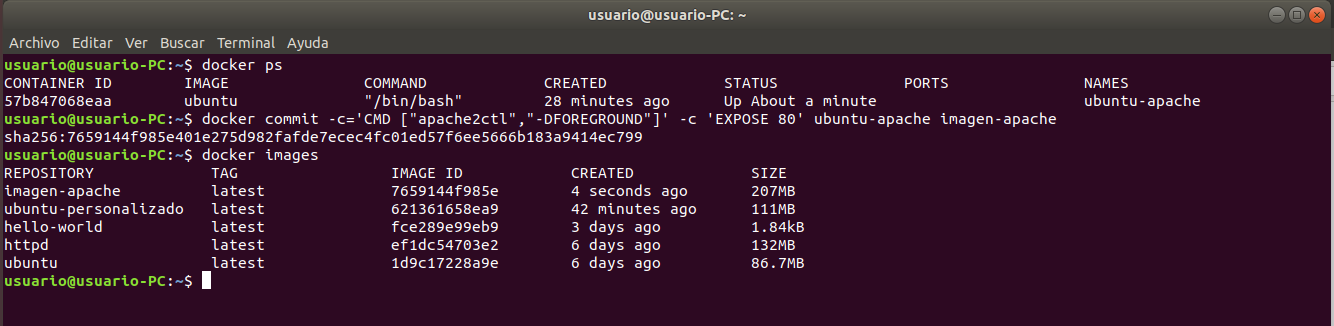
\includegraphics[width=\linewidth]{Trabajo/RecursosEducativos/RE05_Docker/Caso_resuelto/REDocker_Caso1.png}
	\vspace{-0.2cm}
	\caption{Creación imagen personalizada}
	\label{fig:DockerCaso1}
\end{figure}

Teniendo la imagen llamada imagen-apache disponible se procede a crear un nuevo contenedor basado en ella, utilizando el siguiente comando:

\begin{commandshell}
docker run --name nuevo-apache -d -p 8080:80 imagen-apache
\end{commandshell}

En el comando utilizado anteriormente resalta lo siguiente:
\begin{itemize}
    \item -d: Ejecuta el contenedor en segundo plano.
    \item -p 8080:80 : Permite que el puerto 80 del contenedor sea accedido a través del puerto 8080 del host.
    \item --name nuevo-apache: Nombre del contenedor.
\end{itemize}

En la figura \ref{fig:DockerCaso2} se muestra el proceso de creación y verificación del funcionamiento del contenedor llamado nuevo-ubuntu.

\begin{figure}[!hbtp]
	\centering
	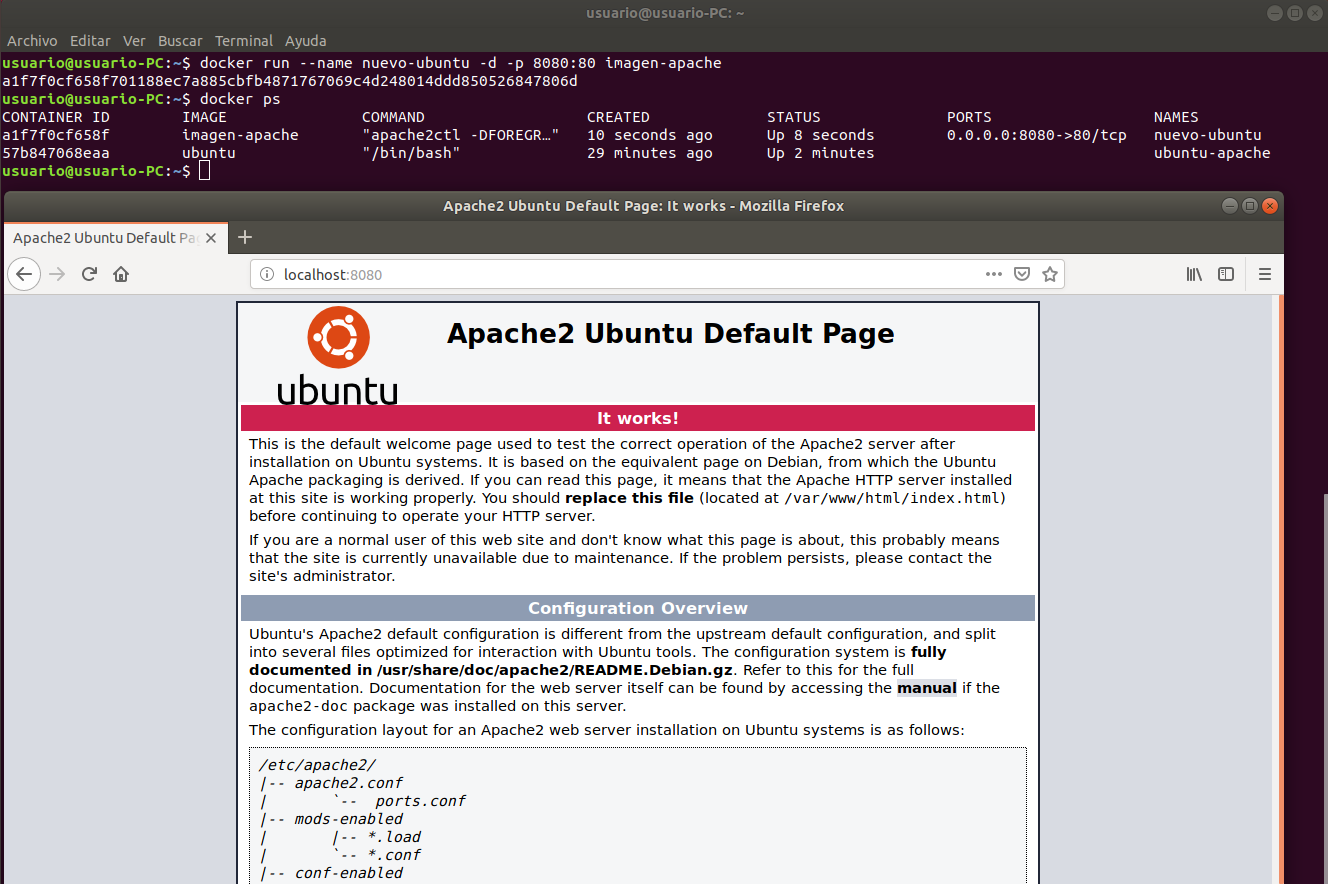
\includegraphics[width=\linewidth]{Trabajo/RecursosEducativos/RE05_Docker/Caso_resuelto/REDocker_Caso2.png}
	\vspace{-0.2cm}
	\caption{Creación imagen personalizada}
	\label{fig:DockerCaso2}
\end{figure}